\documentclass[Rapport]{subfiles}
\begin{document}

\section{Resultat}
\label{sec:Resultat}

% Inledande text?

I den föregående sektionen om optimise beskrivs hur optimeringen sker.
I det här avsnittet beskrivs hur kod ser ut efter optimering och 
olika tidsjämförelser sker med och utan optimise. 
Vi testar CBN-semantiken med anropsstack.

Det finns massor av platser i kod där optimise kan placeras, men alla dessa är tyvärr 
inte bra val. Det finns flera fallgropar att undvika för få ut så stor 
prestandavinst som möjligt. Vi ska illusterar detta igenom att undersöka ett 
något större exempel, en raytracer.

\subsection{Raytracer}


En raytracer är ett program som målar upp en bild genom att skicka ut strålar från en punkt
i ett rum och sedan se vad varje stråle träffar
\footnote{Att jämföra med hur våra egna ögon fungerar. 
          Fast vi skickar inte ut strålar.}.
Utifrån detta kan den sedan bygga upp en bild. Vi har implementerat
en mycket enkel sådan, där rummet består av en djupsorterad lista av tvådimensionella objekt.
Varje objekt beskrivs av en funktion, $Punkt \mapsto Bool$, där den booleska
variabeln svarar på frågan `Ligger den här punkten inom objektets ramar?'.

För att underlätta ges de tänkta typerna för funktionerna som en kommentar ovan definitionen.
En cirkel med radie \ic{1.0} och en kvadrat med sidorna \ic{2.0} defineras:
\begin{codeEx}
-- type Shape = Pos -> Bool
-- circle, square :: Shape

circle p = absSqr p <. 1.0;
square p = case p of
    { Pos x y -> x >. -1.0 && x <. 1.0
              && y >. -1.0 && y <. 1.0
    };
\end{codeEx}

Vi har sedan en rad kombinatorer för att bygga upp mer komplexa objekt:
translation, skalning, rotation, och olika sätt att sammanfoga flera objekt.

\begin{codeEx}
-- translate, scale :: Pos -> Shape -> Shape
translate dp s p = s $ posSub p dp;
scale     dp s p = s $ posDiv p dp;

-- rotate :: Double -> Shape -> Shape
rotate theta s p = s $ polar (abs' p) (arg p +. theta);

-- union, minus, intersect :: Shape -> Shape -> Shape
union     s t p = s p || t p;
minus     s t p = s p && not (t p);
intersect s t p = s p && t p;
\end{codeEx}

Vi ser att ett komplext objekt bara blir en sammasättning av booleska 
funktioner, vilket vid optimering kan infogas och till slut bli ett enda stort \kw{case}-träd. 
Låt oss börja med att betrakta en enkel figur, en fyrkant med sina sidor
nerskalade till 1.0.

\begin{codeEx}
box  = scale (Pos 0.5 0.5) square
box' = optimise box
\end{codeEx}

\ic{box} är nu en funktion från \kw{Pos} till \kw{Bool}. Det är vid sådana halvt applicerade funktioner
som optimise skiner. Optimise kommer bland annat att infoga funktionsanrop och kasta bort onödiga \kw{thunkar}. 
Såhär ser den optimerade boxfunktionen ut i STG-kod. Den är lite svår att tyda 
eftersom alla aktiveringspostindex står med:
 

\begin{codeEx}
  box' = FUN <2> (p -> case <0,p> of
     { Pos x1 y1 -> let
         { i.cc = THUNK [i.bu <1,x1> i.bw] 3 (<0,f> <1,x1> <2,x2>)
         } in let
           { i.cd = THUNK [i.bu <2,y1> i.bx] 3 (<0,f> <1,y1> <2,y2>)
           } in let
             { i.cg = THUNK [<3,t.a> <4,t.b>] 4 (let
                 { t.ad = THUNK [<0,x>] 2 (let
                     { t.ae = CON (D# 1.0)
                     } in <. <0,x> <1,t.ae>)
                 } in let
                   { t.af = THUNK [<1,y>] 3 (let
                       { t.ag = THUNK [<0,y>] 2 (let
                           { t.ah = CON (D# -1.0)
                           } in >. <0,y> <1,t.ah>)
                       } in let
                         { t.ai = THUNK [<0,y>] 2 (let
                             { t.aj = CON (D# 1.0)
                             } in <. <0,y> <1,t.aj>)
                         } in and <1,t.ag> <2,t.ai>)
                   } in and <2,t.ad> <3,t.af>)
             } in case <1,x1> of
               { D# i.c -> case <6,i.c> /.# 0.5 of
                   { {i.e} -> case <7,i.e> >.# -1.0 of
                       { {i.e} -> case <8,i.e> of
                           { True  -> <5,t.ac>
                           ; False  -> $False
                           }
                       }
                   }
               }
     })
\end{codeEx}

Denna version av koden är billig att få fram ur tidssynpunkt och ger ganska
mycket snabbare kod som vi ska se i nästa underavsnitt. Om vi använder \kw{casebranches}
på samma exempel får vi ännu finare kod som bara består av en rad med \kw{case}-satser,
men optimeringen tar mycket längre tid:

\begin{codeEx}
  i.bp = FUN <2> (p -> case <0,p> of
   { Pos x1 y1 -> case <1,x1> of
      { D# i.c -> case <3,i.c> /.# 0.5 of
         { {i.e} -> case <4,i.e> >.# -1.0 of
            { {i.e} -> case <5,i.e> of
               { True  -> case <4,i.e> <.# 1.0 of
                  { {i.e} -> case <6,i.e> of
                     { True  -> case <2,y1> of
                        { D# i.c -> case <7,i.c> /.# 0.5 of
                           { {i.e} -> case <8,i.e> >.# -1.0 of
                              { {i.e} -> case <9,i.e> of
                                 { True  -> case <8,i.e> <.# 1.0 of
                                    { {i.e} -> <10,i.e>
                                    }
                                 ; False  -> $False
                                 }
                              }
                           }
                        }
                     ; False  -> $False
                     }
                  }
               ; False  -> $False
               }
            }
         }
      }
   })
\end{codeEx}


Så länge man håller sig till en enda färg kan alla tänkbara figurer modelleras
med objekt i vår implementation. Men när man börjar intressera sig för olika färger krävs det
flera objekt. Vi har valt att se varje objekt som ett par
av en färg och en funktion som säger om en punkt ligger innanför objektets ramar. 
Vi placerar sedan alla våra sådana par i en lista där första elementet är det
objekt som ska målas upp närmast betraktaren. 

Vi har sedan en en funktion som givet en lista av par av färger och funktioner
ger oss vilken färg en viss punkt har. Vi kallar denna funktion för
\ic{shapes}. Till sist har vi en lista av listor av positioner som ger alla
punkter som \ic{shapes} ska köras på och alltså upplösningen för bilden.

\begin{codeEx}

-- screen :: Double -> Double -> [[Pos]]
screen szX szY = let { xs = fromTo -1.0 (2.0 /. (szX -. 1.0)) 1.0
                     ; ys = fromTo -1.0 (2.0 /. (szY -. 1.0)) 1.0
                     }
                 in map (\x . map (\y . Pos x y) ys) xs;

pic = map (map (shapes [Tuple box red])) $ screen x y;

\end{codeEx}

Om man nu vill optimera ovanstående finns det ett par olika tillvägagångssätt. Det som varit mest effektivt när vi testat är att optimera varje objekt för sig. Det är även så vi gör i våra testresultat, fast för en mycket mer komplex scen, tex: 
\begin{codeEx}
map (map (shapes 
             [ Tuple (optimise box) red
             , Tuple (optimise sky) blue 
             ])
         ) $ screen x y;
\end{codeEx}

\subsubsection{Körningstider}


\begin{figure}[H]
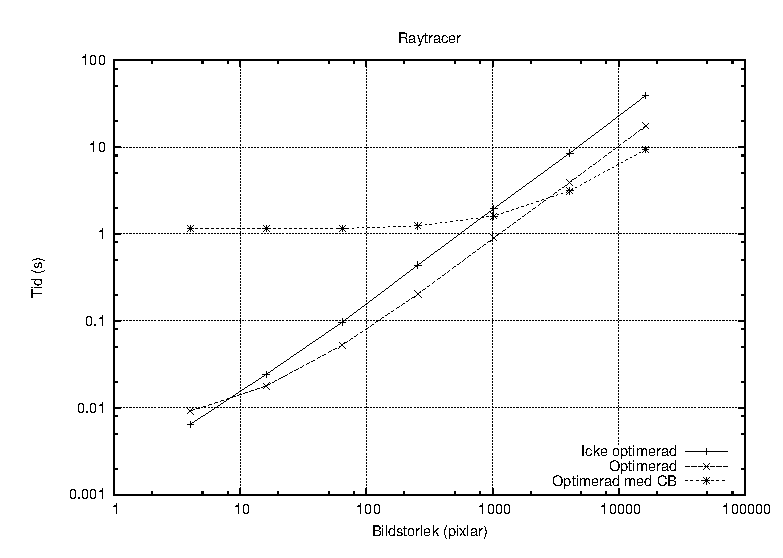
\includegraphics{shapes.eps}
\caption{Logaritmisk graf över körningstid för raytrace, med och utan optimise.}
\label{fig:Resultat:shapes:graf}
\end{figure}

I grafen ser vi att optimeringen utan \kw{casebranches} (CB) påslaget är en
magnitud snabbare per bildstorlek (antal pixlar) redan vid ett lågt antal pixlar.
Vid den lägsta storleken kan vi se hur mycket tid som går åt till optimeringen,
men denna tid är konstant och blir snart en obetydande del av körningstiden. För
större bilder ser det ut som att den optimerade versionen är en konstant gånger
snabbare per pixel, vilket är precis det resultat som vi förväntar oss.

Vi ser även att \kw{casebranches} har en mycket hög körningstid oavsett antalet pixlar. 
Det beror på att optimise kommer att infoga in alla möjliga \kw{case}-grenar, 
vilket vid komplexa figurer kan ge upphov till exponentiellt beteende.
För stora bilder vinner man ändå på att använda casebranches, eftersom optimeringstiden
också här ändå bara är konstant och vid körning behöver inga uppslag i heapen eller icke-primitiva funktionsanrop utföras. 


\subsection{Powergrafer}
Nästa exempel kommer från den välkända \kw{power}-funktionen där vi upphöjer varje element i en lista med tal till ett givet heltal. 
\begin{codeEx}
main = map (optimise (exp getInt)) getIntList;

exp to x = case to == 0 of
    { True  -> 1
    ; False -> x * (exp (to - 1) x)
    };
\end{codeEx}

Låter vi \ic{getInt} $\mapsto 4$ kommer följande kod generas.

\begin{codeEx}
  i.m = FUN <2> (x -> case <0,x> of
    { I# i.c -> case prim("*")# <1,i.c> 1 of
       { {i.e} -> case prim("*")# <1,i.c> <2,i.e> of
          { {i.e} -> case prim("*")# <1,i.c> <3,i.e> of
             { {i.e} -> case prim("*")# <1,i.c> <4,i.e> of
                { {i.e} -> let
                   { i.bd = CON (I# <5,i.e>)
                   } in <6,i.f>
                }
             }
          }
       }
    })
\end{codeEx}

Notera hur vi endast utför mönstermatchning en gång på \ic{x}, och hur det bara finns 
primitiva funktionsanrop kvar. Optimise klarar sig så pass bra att \kw{casebranches} inte 
gör någon som helst skillnad.


\subsubsection{Körningstider}


\begin{figure}[H]
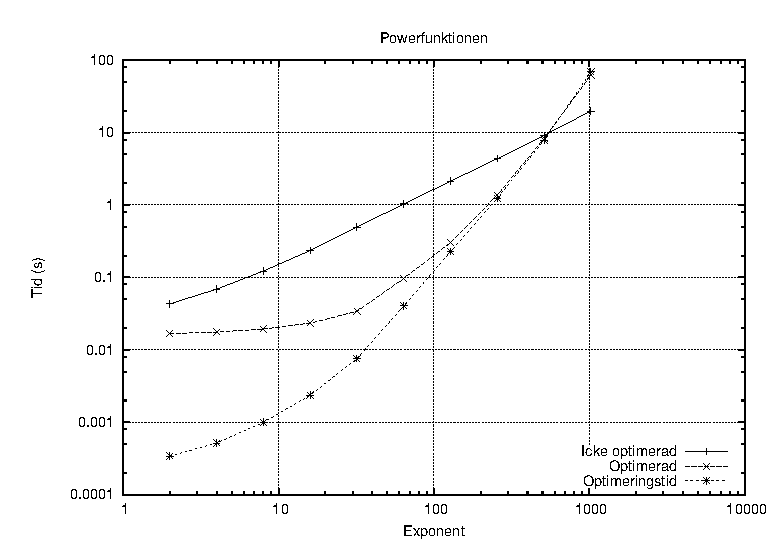
\includegraphics{power.eps}
\caption{Logaritmisk graf över körningstid för power med känd exponent.
Med och utan optimise.}
\label{fig:Resultat:shapes:graf}
\end{figure}

I början presterar den optimerade funktionen precis som förväntat, men runt \ic{exp 50}
börjar optimise ta betydligt längre tid på sig. Detta beror på att optimise inte kör med linjär tidsåtgång i detta fallet. 

% Kanske borde förklaras bättre. Varför har den inte det? :(
\begin{comment}
    \subsection{Expertis}
    Optimise är bra på:
    \begin{itemize}
        \item infogning av funktioner och primitiver
        \item optimera casebranches
        \item beräkna konstantuttryck i en PAP och klistra in resultatet
                 ( detta kan också lösas med full laziness i vissa fall - (vilka?))
    \end{itemize}

    \subsection{Noteringar}

    \NOTE{ 

    \begin{itemize}
        \item Jämför hur kod ser ut före och efter optimering. Förklara lite vad som har gjorts.
            \begin{itemize}
                \item Power har använts som löpande exempel, så vi skulle kunna visa det
                      här också.
                \item Andra program. Förslagsvis något av de lite större exempelprogrammen om vi
                       får dem att fungera bra och kan presentera det på ett vettigt sätt.
                        Shapes, regexp
            \end{itemize}
        \item Jämför snabbheten hos program med och utan optimering (benchmarks)
            \begin{itemize}
                \item Med och utan callstack för att visa hur mycket snabbare resultat det gav oss?
                \item scatterplot för en större mängd program (el. körningar)
        \item Tester med olika stora indata,
            tex listlängd pa x-axeln,
                procentuell ökning på y-axeln,
                upphöjttill-inten på z-axeln.
            
        Antagligen tillräckligt  intressant att ha 2 st av dem, tex optfunktionens storlek mot tid
                                          samt inputens storlek mot tid.
            \end{itemize}
        \item Jämför kodstorlek, komplexitet hos optimise
        \item Hur stor del av tiden går åt till att köra optimise? En graf skulle kunna visa
          detta på ena axeln och listlängd på andra axeln, för att illustrera att
          en optimerad funktion måste köras många gånger för att man ska vinna något på det.

                                          


    \end{itemize}

    }
\end{comment}


\end{document}

